% !TEX root = ../Dissertation.tex
%===================================================================================================

\chapter{Data Collection}




\section{B cells are developing in the NOD thymus}
The reason for B cells being present in the thymus is unknown. 
The potential mechanisms, as outlined in \toref{somewhere in background} are B cells developing from progenitors within the thymus or B cells are being released prematurely from the bone marrow and migrating to the thymus where they continue and complete their development.
In order to investigate the potential for development of B cells within the thymus further, methods such as flow cytometry, magnetic-activated cell sorting (MACS) and polymerase chain reaction (PCR) were used to assess the possibility for intrathymic B cell development.
The process of investigation proceeded as follows:
\begin{enumerate}
\item FLow cytometry was used to look for early progenitors from the haematopoeitic stem cell (HSC) stage, through to the B cell-biased (BLP) stage in the thymus. \toref{relevant subsection}
\item Flow cytometry was used to look for developing B cells at the pro and pre B cell stages in the thymus \toref{relevant subsection}
\item Polymerase chain reaction was used to investigate the presence of transcription factors and genes driving B cell development in the  thymus. \toref{relevant subsection}
\end{enumerate}

Each will be discussed in the relevant sections below.

\todo{here, write about the potential for B cells developing in the thymus and the methods used to investigate it. Could say that the methods involved carrying out magnetic cell sorting and this required a lot of optimisation to get best efficiency/yield}

\subsection{Magnetic-assisted cell sorting optimisation}

Due to the small size of progenitor populations in comparison to mature cell populations in the thymus, it was first necessary to deplete the thymus of the majority of mature cells before looking for progenitors.
For depletion, magnetic-activated cell sorting (MACS) was used.
There are many different kits available and the decision on which to use for the experiments was taken after investigating the efficiency and yield from Miltenyi beads and columnms, and Qiagen anti-rat beads \todo{name of Qiagen beads}

Firstly, Miltenyi columns and lineage depletion beads were tested to assess their efficiency. 
\fig{add figure showing efficiency of beads/columns here}.
To start with, only one round of depletion was carried out which gave an efficiency of \todo{look at efficiencies}.
This efficiency was improved to \todo{add efficiency of 2 rounds} when two rounds of depletion were carried out \fig{2 round miltenyi lineage depletion}. 
\begin{figure}
	\begin{subfigure}{\textwidth}
	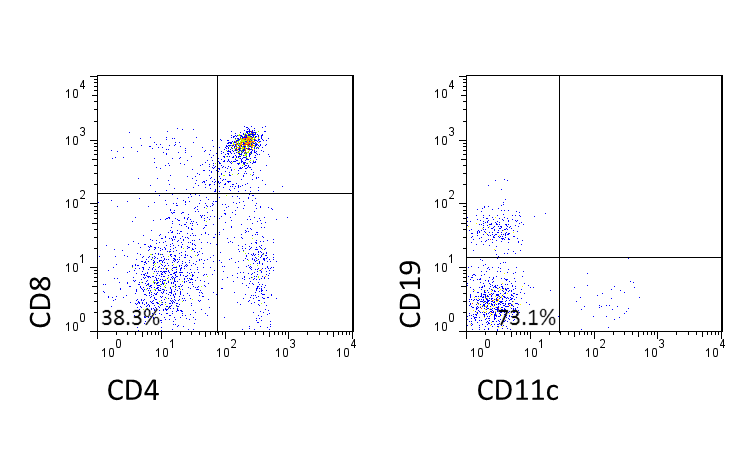
\includegraphics[width=\textwidth]{Figures/1rounddepletion.png}
	\caption{One round of depletion using Miltenyi lineage depletion beads and columns}
	\end{subfigure}
	\hfill
	\begin{subfigure}{\textwidth}
	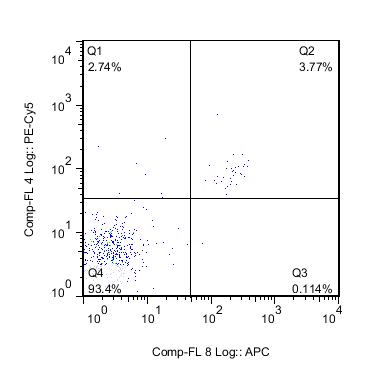
\includegraphics[width=0.3\textwidth]{Figures/2rounddepletion.png}
	\caption{Two rounds of depletion using Miltenyi lineage depletion beads and columns}
	\end{subfigure}
	\hfill
	\begin{subfigure}{\textwidth}
	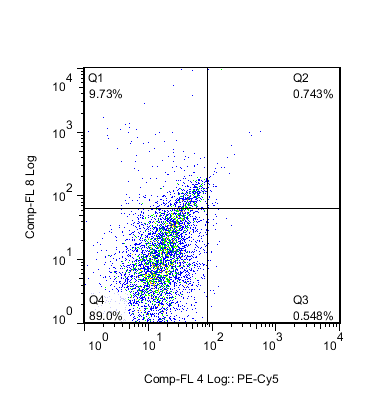
\includegraphics[width=0.3\textwidth] {Figures/Qiagenbeads.png}
	\caption{Qiagen beads}
	\end{subfigure}
\end{figure}
However, while this method gave a very pure sample with very few mature cells remaining, the yield was not very good.

Since the point of the depletion was just to reduce the quantity of mature cells so that the progenitor populations could be seen by flow cytometry, it was more important for the experiment that there was a lot of cells to interrogate rather than them being very pure.
Therefore, Qiagen beads were tried and as shown, \fig{figure of Qiagen depletion}, while the purity was not as good as the Miltenyi beads \todo{efficiency of Qiagen beads}, the yield was much improved.
This was a better balance for the experiment, therefore, Qiagen beads were used.

\subsection{Early B cell progenitors are present in the NOD thymus}
\todo{analyse results comparing NOD/KO/B6 data to see if the presence of BLPs is normal in NOD}
Once the method of lineage depletion was decided on, it was then possible to move forward to investigating the early progenitor populations in NOD, NOD KO and B6 thymi.
BLP presence was of particular interest as differences in populations between strains of mice could suggest whether the increase in B cells in the NOD thymus was as a result of processes before or after this point.
BLPs are thought to be the first cell committed to the B cell lineage therefore if the populations of these cells are different, it could suggest abnormalities in factors driving B cell commitment.


\subsection{Pro and Pre B cells are present in the NOD thymus}

\subsection{CD19+ RAG+ B cells are seen in the NOD thymus}


\subsection{B cell development is dependent on the presence of a mature B cell}
\subsubsection{Transfer experiment - Transfer of NOD thymic cells to B cell KO NOD mice}

\subsection{T cell development looks normal/abnormal in NOD mouse compared to control}
\todo{analyse data to see whether it is normal or abnormal. This is a good control to give an indication of the overall condition of the thymus, preferably over time to see how it changes as mouse ages with normal physiological atrophy of the thymus}

\subsection{Conclusion}




\section{There is potentially a population of cells expressing both T and B cell receptors in the NOD thymus}

\subsection{A large proportion of RAG+CD19+ cells in 4 and 7 week old NOD thymus also express CD4 and CD8}
An incidental finding whilst analysing data from the NOD-RAG-GFP mice looking for CD19+RAG+ cells in the thymus, showed that a large proportion of these cells were also expressing CD4 and CD8. \fig{add figure here showing gating LCs, SCs, RAG+, CD19+, CD4 v CD8}. 
This finding was seen in NOD mice at both 4 and 7 weeks of age.
The gating pattern is shown in \cref{fig:RAGposDP}
\todo{add some data/graph/statistics to show significance, whether there is a difference between the ages etc}

\begin{figure}	
	\begin{subfigure}{\textwidth}
		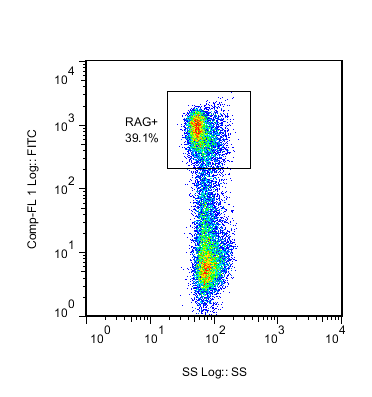
\includegraphics[width=0.3\textwidth] {Figures/RAGposthy1241014.png}
		\hfill	
		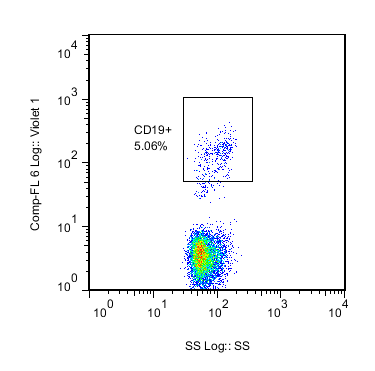
\includegraphics[width=0.3\textwidth] {Figures/RAGCD19posthy1}		
		\hfill	
		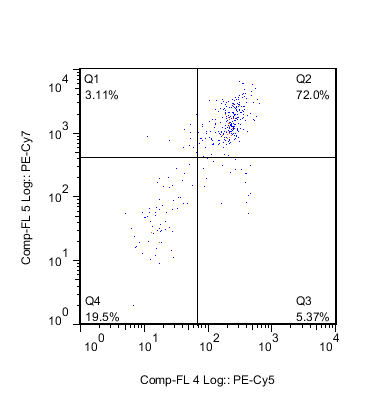
\includegraphics[width=0.3\textwidth] {Figures/RAGCD19CD4CD8posthy1}
		\caption{Final testing}
		\label{fig:RAGposDP}
	\end{subfigure}
\end{figure}



\subsection{Elevated level of CD8 on CD19+ cells in the thymus}

\subsection{IgM+TcRb+ cell presence}
Following on from this finding, the whole thymus was then interrogated for cells which were expressing both T and B cell receptors, in this case TcRb and IgM. 
This was done by carrying out flow cytometry on thymus samples from NOD mice of various ages.


\todo{include isotype control data}

\subsection{RAG+IgM+TcRb+ cell presence in the NOD thymus}

\subsection{Conclusion}




\section{Potential contribution of thymic B cells to T1D}

\subsection{Pilot study to track movement/homing of thymic B cells on transfer into recipient mice}
\todo{where B cells traffic to could give indication of their role in T1D. Also, use of GFP as  a marker. However, numbers were very small so analysis difficult. Needs to be done again in the future. Comment on whether it may be possible and what would need to change to make it work. Also decide on which transfer experiment I am referring to.. NOD to KO or GFP to NOD...}
In order to look at the potential impact that thymic B cells may be having on the pathogenesis of T1D, a pilot study looking at the migration of donor thymic B cells following intravenous injection into recipient mice was set up. 
At time points of 7 and 11 days post injection, recipient mice were sacrificed and their thymus, spleen, bone marrow, pancreas, pancreatic lymph node and lateral axillary lymph node were all analysed by flow cytometry.
The tissues to analyse were chosen for the following reasons:
\begin{itemize}
\item Thymus - The thymus is the tissue where the donor cells were taken therefore it was included in analysis to see if the donor cells would migrate back to the thymus in the recipient cells.
This would give the impression that thymic B cells have specific properties which allow them to traffic back to the thymus.
For example, they may have specific cytokine sensitivity which results in being able to home back to the thymus following transfer.
\item Spleen - The spleen was included for analysis as this is the normal site of B cell maturation.
Therefore it was of interest to see if thymic derived donor cells would move here like conventional B cells do to finish development.
\item Bone marrow - The bone marrow is the normal site of B cell development and therefore was included to see if the developing donor B cells would preferentially to here to develop in the same way as conventional B cells
\item Pancreas - The pancreas contains the Islets of Langerhans which are destroyed in T1D through T and B cell mediated attack.
Pancreatic tissue was therefore analysed to see if thymic B cells migrate to here preferentially upon transfer into recipient mice.
If so, it may indicate that thymic B cells could have a direct role in the pathogenesis of the disease.
\item Pancreatic lymph node - The PLN is where antigen-presenting cells move to from the pancreas in order to activate T cells.
In T1D, APCs move from the pancreatic islets to the PLN carrying islet antigens and therefore the PLN is in an inflammatory state.
This tissue was therefore included to look at the status of the lymph node to compare it to the control axillary lymph node.
\item Lateral axillary lymph node - This tissue was analysed as a control to compare to the PLN.
Whereas the PLN should be inflamed in T1D, the lateral axillary lymph node should not and can therefore show that any inflammation in the PLN is localised and is not as a result of inflammation throughout the body.
\end{itemize}

\subsection{Autoantibody production}

\subsection{Conclusion}

